\part{Du traitement de texte à l'encodage} 

\chapter[Préparation à l'encodage]{Préparer le traitement de texte à l'encodage en XML}

\vspace*{\stretch{1.3}} 
\par Les actes du corpus étant édités aux formats ODT et docx, il s’agit dans un premier temps de les nettoyer, c’est-à-dire de les préparer à un encodage, afin de permettre aux chercheurs de manipuler le corpus. XML (Extensible Markup Language) est un langage de balisage qui révèle la structure et la sémantique des données, conçu pour la description des documents textuels, et en ce sens adapté pour l'édition critique. Le recours au langage de balisage XML permet une structuration des éléments textuels à l'aide de balises, ce que le traitement de texte ne permet pas. Depuis 1998, XML est un langage libre et documenté qui facilite la lisibilité des données, leur échange et leur migration vers d’autres plateformes, logiciels et formats. C'est aujourd'hui un standard du W3C\footnote{World Wide Web Consortium : communauté internationale qui développe des normes ouvertes pour assurer la croissance à long terme du Web.} qui comporte différents formats comme la TEI (Text Encoding Initiative) pour l'encodage de documents patrimoniaux.
\vspace*{\stretch{0.7}} 
\newpage 

\section{Le recours à un langage de balisage}
\label{II.3.1}

\par Le chercheur en philologie Claus Huitfeld défini le balisage comme \og l'usage de chaînes de caractères réservés, insérées dans des séquences de caractères dans des fichiers de documents numériques, afin de dénoter ou de signaler des caractéristiques d'un document qui ne peuvent pas être transmises par des caractères représentant directement leur contenu verbal \fg \footnote{\og Systèmes de balisage de textes et édition critiques\fg, in : \cite{apollonEditionCritiqueEre2017}}. Le terme balisage renvoie à des marqueurs spéciaux permettant de signaler certaines propriétés du document numérique (ponctuation, notes…) via un ensemble de balises\footnote{\cite{apollonEditionCritiqueEre2017}}. L’édition scientifique actuelle fait appel à des méthodes de publication informatisées qui induisent du balisage. Les systèmes de traitement de texte ou de publication sur le web les plus utilisées actuellement disposent d’un système de balisage en \og arrière-plan \fg \space que l'usager n'a pas à gérer : il intervient directement sur le document via une mise en page visuelle (WYSIWYG : \og what you see is what you get \fg\footnote{\og Ce que vous voyez est ce que vous obtenez\fg : l'utilisateur voit directement le résultat de sa saisie.}). Ces outils sont utiles pour l'affichage à l'écran ou l'impression papier, mais dès lors que l'on souhaite proposer des outils de recherche performants, de comptage, ou encore d'analyse, il devient nécessaire d'effectuer un balisage généralisé du texte. Différents langages de balisage existent et comprennent une syntaxe, un vocabulaire contrôlé, des méthodes, des pratiques et des outils associés\footnote{\og Systèmes de balisage de textes et édition critiques\fg, in : \cite{apollonEditionCritiqueEre2017}}. 
\newline 

\begin{figure}[ht]
    \centering
    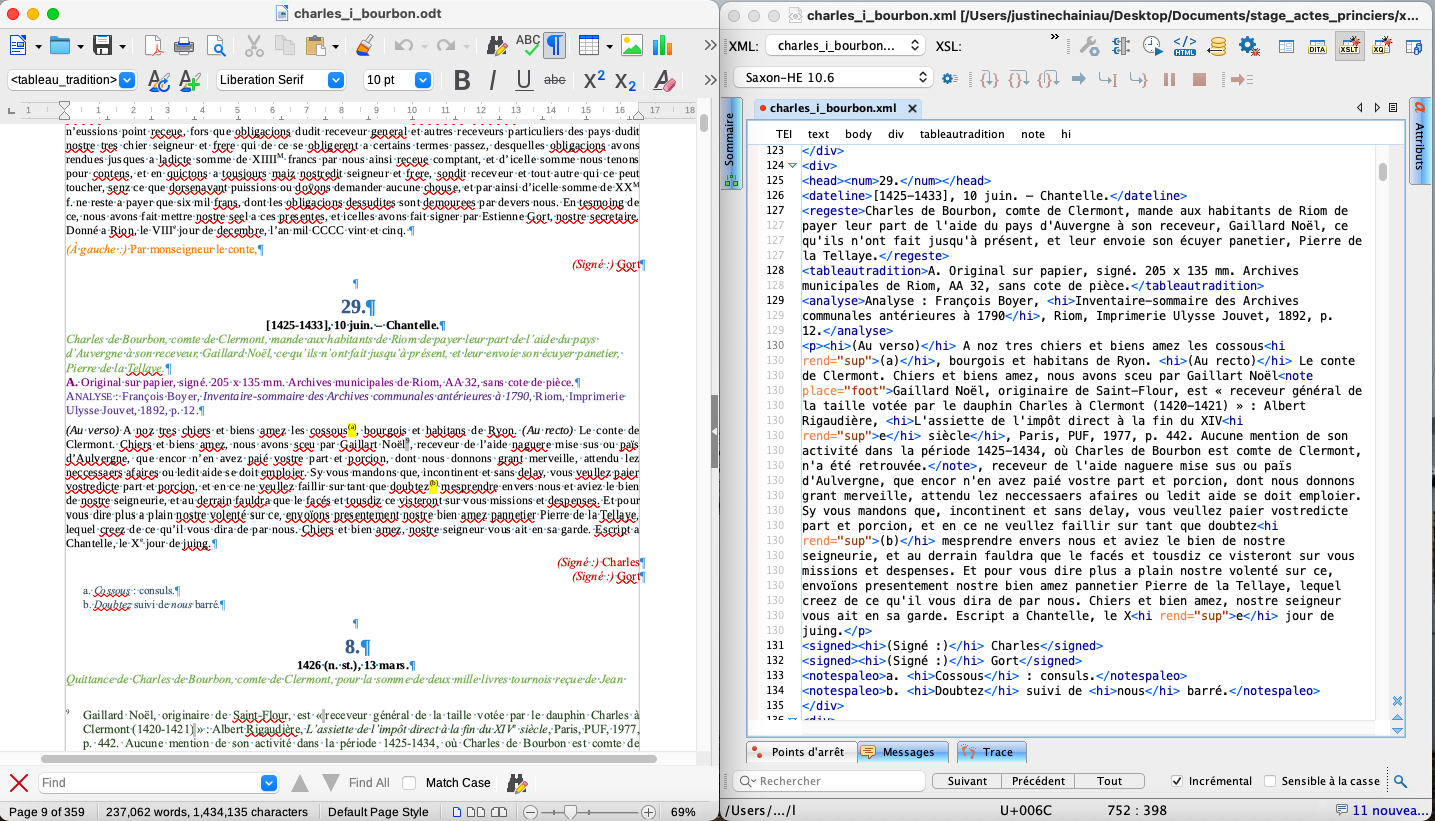
\includegraphics[scale=0.3]{front/images/odt_vs_xml.png}
    \caption{Traitement de texte et encodage de l'acte n°29 daté du 10 juin 1425-1433.}
    \label{fig:odt_vs_xml}
\end{figure}
\newpage 

\par Le langage XML est le plus approprié pour l’édition numérique. Contrairement au langage HTML (HyperText Markup Language) dont les balises définissent l’apparence des données (titres, paragraphes), les balises du langage XML définissent la structure et la signification sémantique des données, ce qui permet leur réutilisation. La particularité du XML est que son affichage nécessite une interprétation, soit une transformation du document. Le document XML est alors transformé via des feuilles de style XSL (Extensible stylesheet language)\footnote{Extensible stylesheet language : langage des feuilles de style associées à XML.} en document HTML pour une disponibilité sur le web ou en PDF pour une impression de qualité. Cette possibilité de présentation dans une variété de formats sans qu'il soit nécessaire de modifier le code assure l'intégrité des données. En effet, la conversion d'un document produit sous traitement de texte peut être difficile, manquer de fiabilité. De plus, les formats propriétaires ne sont pas documentés publiquement (usage commercial) et comportent un risque d’obsolescence qu’il est important de prendre en compte lorsque l’on souhaite produire un travail pérenne. Ainsi, l’un des principaux avantages du balisage généralisé est son interopérabilité, qui garantit une utilisabilité future. Dans le cadre de la recherche en sciences humaines et sociales, de l’édition en particulier, il est primordial de faciliter l'échange et la réutilisation des documents numériques et d’assurer leur conservation sous une forme qui les rend accessibles à la recherche. Un autre avantage du balisage généralisé est son adaptabilité à différents projets d'édition. Pour cela, différents langages XML ont été développés. 
\newline 

\par En 1994 sont publiées les Recommandations méthodologiques pour le balisage et l'échange de textes électroniques de la TEI\footnote{Text Encoding Initiative : consortium qui élabore et maintient collectivement une norme pour la représentation des textes sous forme numérique : \url{https://tei-c.org/}.}, soit un ensemble de balises qui peuvent être combinées et adaptées à des besoins spécifiques\footnote{\og Systèmes de balisage de textes et édition critiques\fg, in : \cite{apollonEditionCritiqueEre2017}}. La TEI est un langage descriptif de balisage adapté à la description fine des différents aspects d’une source, permettant ainsi au chercheur de caractériser les informations utiles à la production d'une édition. Il s'agit d'un ensemble de recommandations pour les chercheurs sur la création de ressources textuelles informatisées et lisibles par des machines, adaptées aux besoins de la recherche et extensibles, puisque ces besoins changent et évoluent\footnote{\cite{burnardQuEstceQue2015}.}. Les Guidelines de la TEI définissent plusieurs centaines de concepts différents permettant une description scientifique et sémantique d’un texte pour des projets d'édition variés (théâtre, poésie, documents d'archives...). 
\newpage 

\par Les technologies de balisage adaptées à l’édition numérique rendent possible la séparation entre la description et la présentation. Cette différenciation entre la transcription des données textuelles et leur présentation offre à l'éditeur la possibilité de développer de manière distincte l’enregistrement du document et l’affichage des données et des métadonnées le caractérisant (notes, index…)\footnote{\og Éditions critiques et séparation de la description et de la présentation, in : \cite{apollonEditionCritiqueEre2017}}. La technologie remet donc en question les pratiques traditionnelles de l'édition. Les standards de balisage du texte assurent l’interopérabilité des données, contribuent à améliorer la qualité de l'édition et de ses éventuelles révisions, et sont en ce sens novateurs. Toutefois, les langages de balisage nécessitent de se familiariser avec leur syntaxe, ce qui peut parfois motiver le choix d’une édition via un logiciel de traitement de texte, comme dans notre cas. 
\newline 

\par Deux possibilités d'encodage s'offrent désormais à nous pour transformer le corpus : manuelle ou automatique. L'encodage manuel étant chronophage, la conversion automatique est plus appropriée. Toutefois, la conversion des ODT en XML sans opérations préparatoires risque de générer une \og dette technique \fg \space (maintenances qui auront une incidence importante sur l'ensemble du projet). En effet, parmi les opérations de traitement des XML obtenus, certaines auraient pu être évitées si la mise en forme du document ODT d'origine avait été améliorée. Pour pallier cette \og dette\fg, il est nécessaire d'harmoniser au maximum les documents en amont.

\newpage 

\section[Utilisation de regex]{Utilisation de regex pour une première structuration du texte}
\label{II.3.2}

\vspace*{\stretch{0.1}} 
\par Le recours à des expressions régulières (regex)\footnote{\cite{ListRegularExpressions}.} s’est révélé opportun pour automatiser le nettoyage des documents\footnote{\cite{UsingRegularExpressions}.}. Les regex sont des chaînes de caractères utilisées pour décrire, dans une syntaxe précise, un ensemble de chaînes de caractères possibles. Leur emploi peut être exécuté à partir de la fonction rechercher/remplacer du traitement de texte. Elles peuvent également être utilisées pour rechercher des caractères non spécifiés ou même invisibles (espaces, sauts de lignes...). Le corpus des actes émis par Agnès de Bourgogne étant moins volumineux, il a tenu lieu d’expérimentation afin de tester la pertinence des regex et leur prochaine application au corpus plus important que représentent ceux de Louis II et de Charles I\textsuperscript{er}. 
\newline 

\par L’utilisation de regex simples a permis dans un premier temps de parfaire la mise en page du document en retirant les doubles espaces, les sauts de lignes ou encore les pages inutiles\footnote{Annexe Liste des regex utilisées.}. Cette étape a été exécutée avec facilité pour le premier corpus relatif aux actes d’Agnès de Bourgogne. Néanmoins, le traitement d’un fichier plus volumineux, comme celui de Charles I\textsuperscript{er}, nous confronte à des problèmes de mise en page. Nous remarquons la présence d’espaces similaires à des tabulations devant les mentions hors teneurs. L’affichage de \og la mise en page \fg \space sur Word a permis de repérer ces anomalies, à savoir l’apparition de mentions \og sur le repli \fg \space par la suite masquées en blanc afin d’aligner les mentions hors teneur en vue de l'impression du mémoire de Master. Le recours à une regex plus ciblée a permis leur suppression et a réglé les problèmes d’indentation. Dans un second temps, les regex ont contribué à améliorer la lisibilité du document. Les notes paléographiques ont bénéficié d’un retour à la ligne et les astérisques faisant office de séparateur des actes ont été supprimées. Seule la numérotation des actes a été retenue, car contrairement aux astérisques, elle est présente dès le premier acte, ce qui évitera un encodage manuel de ce dernier, permettant ainsi d'automatiser totalement le processus. 
\vspace*{\stretch{0.2}} 
\newpage 

\par L'automatisation du nettoyage des données via des regex s’est révélée être une méthode puissante pour uniformiser rapidement les éditions. Néanmoins, certaines étapes du nettoyage ont dû être effectuées manuellement, afin d'éviter une perte de données. C’est le cas tout au long du travail avec les fautes orthographiques qui peuvent être repérées progressivement. Les notes de bas de page présentes dans les dates ont été déplacées à la fin de l'analyse afin d'éviter de surcharger l'encodage. Certaines erreurs trop volumineuses n’ont pas encore été résolues et nécessitent un questionnement. C’est le cas de la présence aléatoire de points à la suite des dates. Il y a aussi des problèmes d’harmonisation des mentions hors teneurs et des signataires qui ne sont parfois pas signalés en amont, ce qui ne permet pas de les identifier et d'intervenir dessus via des regex. 
\newline 

\par Ces deux premières étapes n’ayant pas permis de résoudre tous les problèmes de mise en page et d’uniformisation, les dernières phases du processus auront lieu plus tardivement dans le projet lors de l’utilisation d’autres technologies. La mention \og (Signé :) \fg \space devant le nom de chaque signataire n’étant pas continue, il sera plus simple de l’ajouter ou de la retirer plus tardivement lors de l'encodage en XML à partir d'un script Python. Le nettoyage des données découle donc des différentes phases du projet et est aussi dépendant des formats (ODT, XML) et des technologies utilisées (Python...), même si des étapes peuvent être pensées afin de préparer les données à une conversion.

\newpage 

\section[Proposition de stylage]{Proposition de stylage des actes en vue d’une conversion}
\label{II.3.3}

\par Les logiciels de traitement de texte permettent d'appliquer des styles différents à des parties du texte. Le recours aux regex s'est avéré efficace pour structurer le texte via le stylage des différentes parties des éditions. Un style est un \og ensemble de règles de mise en forme, regroupées, nommées, hiérarchisées et enregistrées, afin de pouvoir être facilement réutilisées en bloc par la suite \fg\footnote{Open Office, \og Utiliser Styles et Modèles
avec OpenOffice.org\fg.}. Ces derniers offrent à l'utilisateur un contrôle de la mise en forme des documents. Le format OpenDocument est une archive ZIP contenant des fichiers XML qui renferment le contenu du document (content.xml), les styles utilisés (styles.xml) et les métadonnées associées au fichier (meta.xml)\footnote{Microsoft, \og Différences entre le format Texte OpenDocument (.ODT) et le format Word (.docx)\fg, \url{https://support.microsoft.com/fr-fr/office/diff}.}. Ainsi, lors de la transformation des documents ODT vers XML, les différents styles associés aux parties des éditions seront interprétés par l’éditeur de code, ce qui permettra de les distinguer dans des balises structurantes. 

\par Toutes les différentes parties des éditions : datation, analyse, tableau de la tradition, mentions hors teneurs, signataires, notes paléographiques et notes de bas de page ont été stylées via des regex\footnote{Annexe Liste des regex utilisées.}. Dans la mesure où la mise en forme de toutes ces parties était relativement normalisée, les expressions régulières ont permis d'identifier les chaînes de caractères ciblées et de les styler. Les styles ont été créés à l'aide de la fenêtre flottante \og Styles et formatage \fg \space qui permet de visualiser les différents styles, de les utiliser, de les modifier, d’en créer ou d'en supprimer. Ces styles ont ensuite été réutilisés et appliqués aux autres documents ODT pour les actes de chaque prince. Nous avons opté pour un stylage coloré afin d'avoir un meilleur aperçu des différentes parties des éditions visuellement. Comme le montre les différents exemples ci-après, le stylage n'a pas été appliqué aux mêmes parties de l'édition selon l'état des actes. Les originaux sont les actes qui ont demandé le plus de stylage dans la mesure où ils comportent toutes les parties de l'édition. 

\begin{figure}[H]
    \centering
    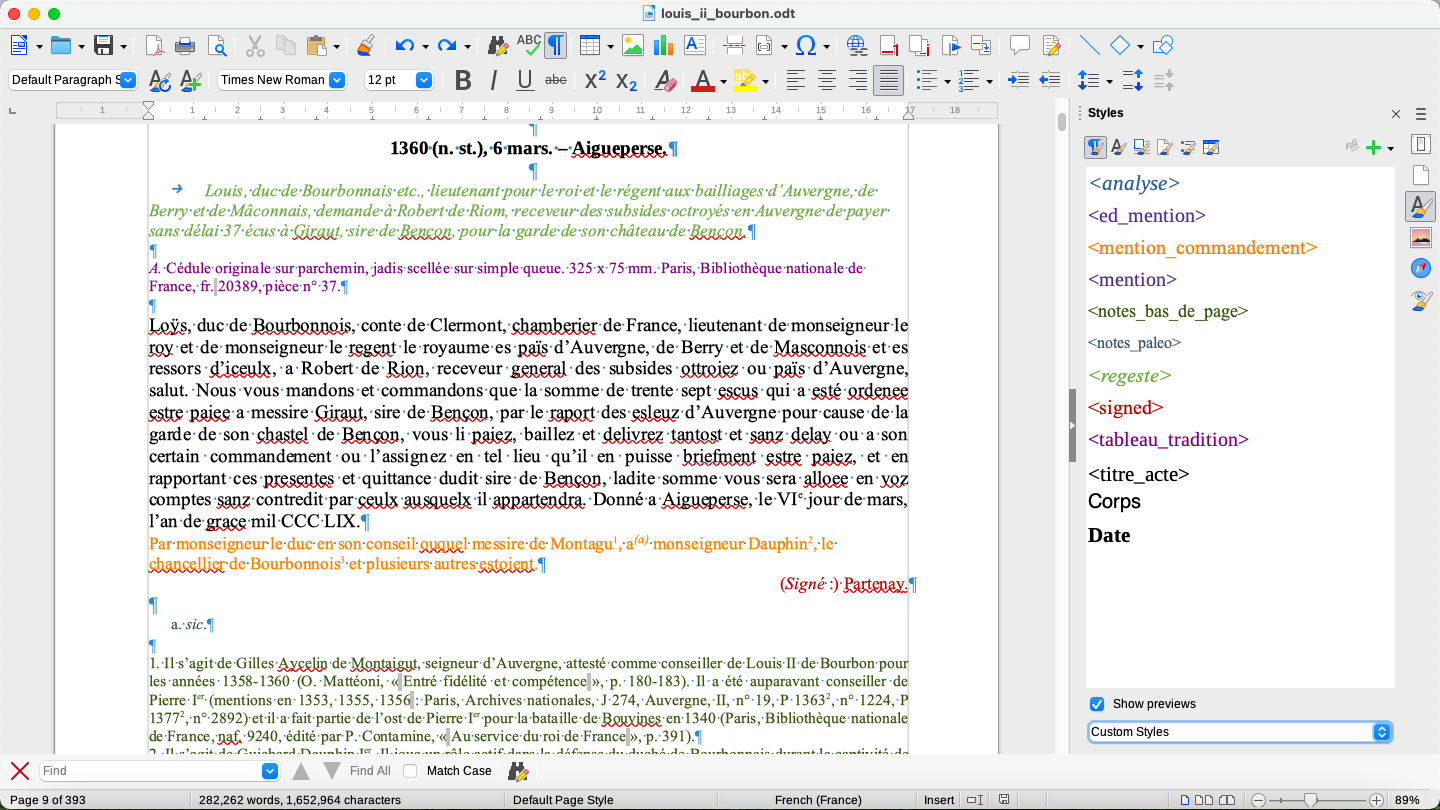
\includegraphics[scale=0.3]{front/images/original.png}
    \caption{Original daté du 6 mars 1360.}
    \label{fig:original}
\end{figure}

\begin{figure}[H]
    \centering
    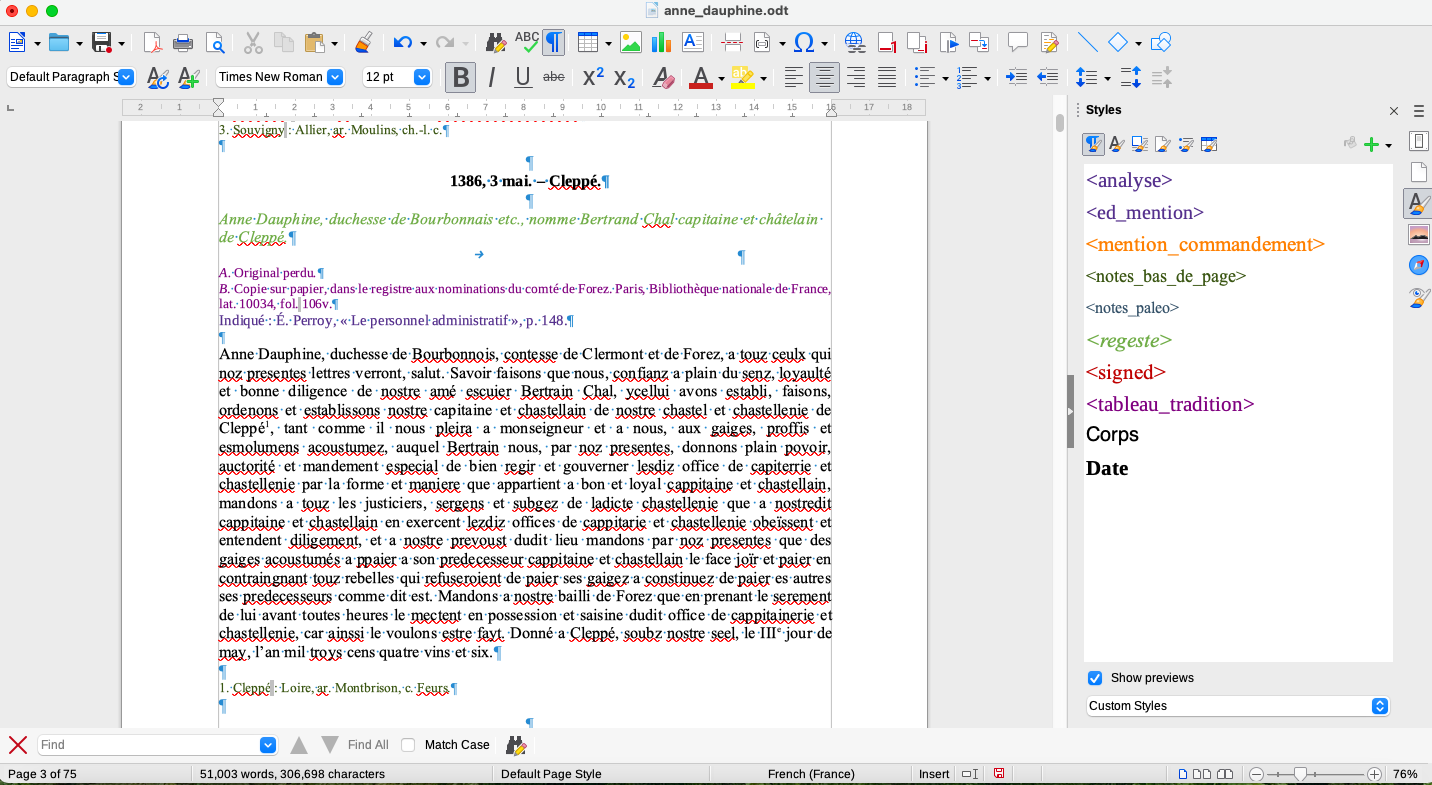
\includegraphics[scale=0.3]{front/images/copie.png}
    \caption{Copie datée du 3 mai 1386.}
    \label{fig:copie}
\end{figure}

\par Les copies et vidimus ne comportent pas de stylage pour les mentions hors teneurs et les signataires puisque l'acte copié ou vidimé est présenté d'un bloc. 

\begin{figure}[H]
    \centering
    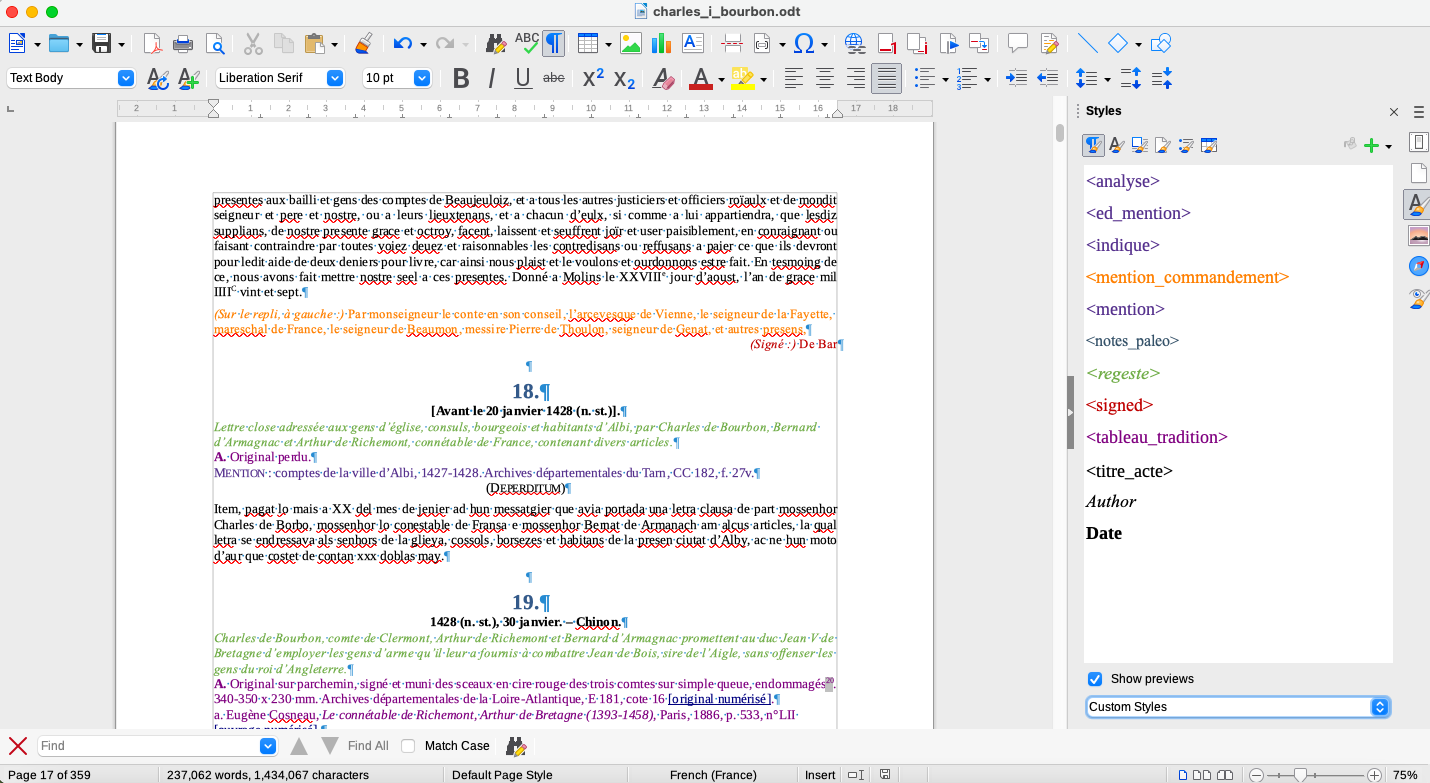
\includegraphics[scale=0.3]{front/images/deperditum_numerote.png}
    \caption{Deperditum numéroté daté d'avant le 20 janvier 1428.}
    \label{fig:dep_num}
\end{figure}

\par Les deperdita sont les actes pour lesquels le stylage est le plus bref et comporte des variations. À l'instar des autres, les éléments de date et d'analyse sont stylés, le tableau de la tradition également, même s'il est très sommaire : il comporte seulement l'indication que l'original est perdu. La mention du deperditum à la suite du tableau de la tradition a cependant nécessité la création d'un style dédié. Le contenu de cette mention est parfois présent, même si ce n'est pas toujours le cas, ce qui peut impliquer des notes. 
\newline 

\par Une autre variation est attribuable aux différents choix d'édition. En effet, les actes transcrits par Jean-Damien Généro, ceux de Charles I\up{er} et d'Agnès de Bourgogne, sont numérotés, ce qui a impliqué la création d'un style titre structurant pour les numéros. Ces étapes ont nécessité de penser des regex plus ciblées et adaptées aux différents corpus. C’est le cas pour les dates dans le corpus de Charles I\textsuperscript{er}. En effet, quelques actes de ce corpus ne sont pas datés de manière précise et obligent à recourir à des adverbes de temps (avant, après et entre). Là où il s'est avéré relativement simples pour les autres corpus, le stylage des analyses des actes de Charles I\textsuperscript{er} a nécessité une harmonisation de ces dernières (normalisation de leur préambule) afin d'automatiser cette étape. Les analyses des premiers actes reflètent la mise en place progressive de la chancellerie de Charles de Bourbon, qui n'est pas encore duc de Bourbon, mais comte de Clermont, et l'évolution de sa titulature. Les corrections se font plus rares après sa nomination, la titulature de “Charles, duc de Bourbonnais et d’Auvergne” étant définitive. Néanmoins, la plupart des corrections apportées ont permis de pallier un problème normatif. Pour beaucoup d’actes, la mention “de Bourbon” après Charles a été oubliée dans les analyses alors qu’elles étaient présentes dans les actes, elle a donc été rajoutée. 
\newpage 

\par L’autre modification concerne les substantifs placés en début d’analyse, que l'on a souvent transformé en verbes, placés à la suite de la titulature du duc. Par exemple, le “consentement donné par Charles de Bourbon” devient “Charles de Bourbon [...] donne son consentement”. Ensuite, le stylage de ces analyses s’est fait par le recours à de nouvelles regex permettant d’attraper les analyses normalisées. Quelques opérations manuelles ont été réalisées pour les analyses uniques, comme pour les testaments ou les ratifications de contrats de mariage. En tout, trente-deux éditions ont fait l'objet d'une modification manuelle. Les mentions hors teneurs situées à la suite du texte ont bénéficié d'une indentation, étape préalable au stylage de toutes les mentions. 
\newline 

\par Néanmoins, le stylage de certains titres ou sections qui n’ont pas été identifiés par les regex a parfois été réalisé manuellement. Une partie du tableau de la tradition mentionnant les éditions au sein du corpus de Louis II n'a pas pu être stylée automatiquement en raison d'une trop grande proximité stylistique avec les notes paléographiques. En effet, la numérotation des éditions est la même que celle des notes paléographiques (a., b., c., etc). De plus, une partie de ces dernières ont, pour des raisons inconnues, échappé au stylage via des regex, ce qui montre leurs limites d'application à des éditions complexes et non normalisées. Le recours à des logiciels spécialisés dans l’édition critique comme \textit{Classical Text Editor}\footnote{\textit{Classical Text Editor}, en ligne : \url{https://cte.oeaw.ac.at/}} aurait permis un gain de temps sur toutes ces étapes et la génération d'une édition standard. Enfin, certaines parties comme le contenu des actes n’ont pu être stylées et structurées grâce à des regex en raison de leur complexité (intitulations) ou de leur typographie et pourront être manipulées plus facilement après la conversion.

\newpage
\thispagestyle{empty}
\mbox{}
\newpage

\chapter{Conversion des fichiers ODT vers XML/TEI}

\vspace*{\stretch{0.2}} 
\par Le format de document texte OpenDocument (ODT) est un format pour les documents textuels modifiables et un des sous-types de la famille ODF pour certaines catégories de contenu, notamment pour les applications de traitement de texte\footnote{OpenDocument Text Document Format (ODT), Version 1.2, ISO 26300-1:2015, en ligne : \url{https://borntocode.fr/latex-comment-inserer-et-customiser-du-code-source/}.}. La structure et le texte d’un fichier ODT sont tous représentés en XML : les paragraphes et les sections sont facilement reconnaissables, tout comme les en-têtes et les pieds de page, ainsi que les constructions de niveau supérieur grâce à l’utilisation cohérente des styles (par exemple, pour les titres), des tables des matières et des index générés automatiquement, et des modèles structurés. Tout le formatage est représenté dans le document ODT et stocké dans des fichiers XML afin de faciliter la séparation du texte et de la structure sémantique des caractéristiques de mise en page. Les formats de traitement de texte tels que l’ODT stockent de nombreuses informations associées au processus de création et d’examen des documents, y compris les modifications. Toutes ces informations seront interprétées lors de la conversion. L’enjeu est de trouver un convertisseur adapté, dont le résultat reflètera le mieux possible l'édition des actes. Plusieurs convertisseurs ont été testés afin de mesurer leur convenance, celle-ci étant essentiellement basée sur la reproduction de l’organisation des documents. 
\vspace*{\stretch{0.1}} 
\newpage 

\section{Les convertisseurs libres}
\label{II.4.1}

\par D'abord, nous avons testé, par curiosité, deux convertisseurs libres. Premièrement, le niveau de structuration après conversion s’est avéré relativement mauvais. \textit{AnyConv} sépare les actes dans des sections, avec un niveau de titre correspondant à leur numéro\footnote{AnyConv : Convertisseur de ODT en XML, en ligne : \url{https://anyconv.com/fr/convertisseur-de-odt-en-xml/}.}. Hormis cela, tous les éléments sont ensuite encodés dans des balises <para> sans distinction aucune ni précision de la typographie ou des styles. 

\begin{figure}[ht!]
    \centering
    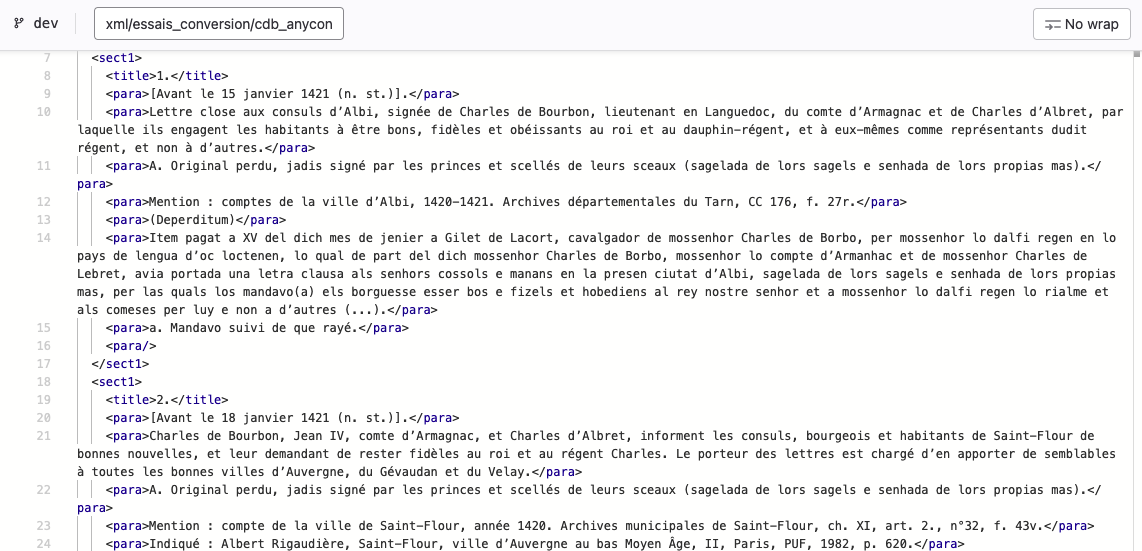
\includegraphics[scale=0.4]{front/images/any_conv.png}
    \caption{Document XML converti avec \textit{AnyConv}.}
    \label{fig:any_conv}
\end{figure}

\par Le second convertisseur libre testé, \textit{Online ODT converter}, affiche dans un premier temps l’ensemble des styles utilisés, ce qui entrave la lecture\footnote{Online ODT converter, en ligne : \url{https://onlineconvertfree.com/convert/odt/}.}. Ensuite, la structuration est assez chaotique : tout le texte est encodé dans des balises <text>. Malgré la reconnaissance des différents styles ODT et leur affichage comme attributs des balises <text>, il n’y a pas de structuration permettant de refléter la séparation des différents actes. 

\begin{figure}[H]
    \centering
    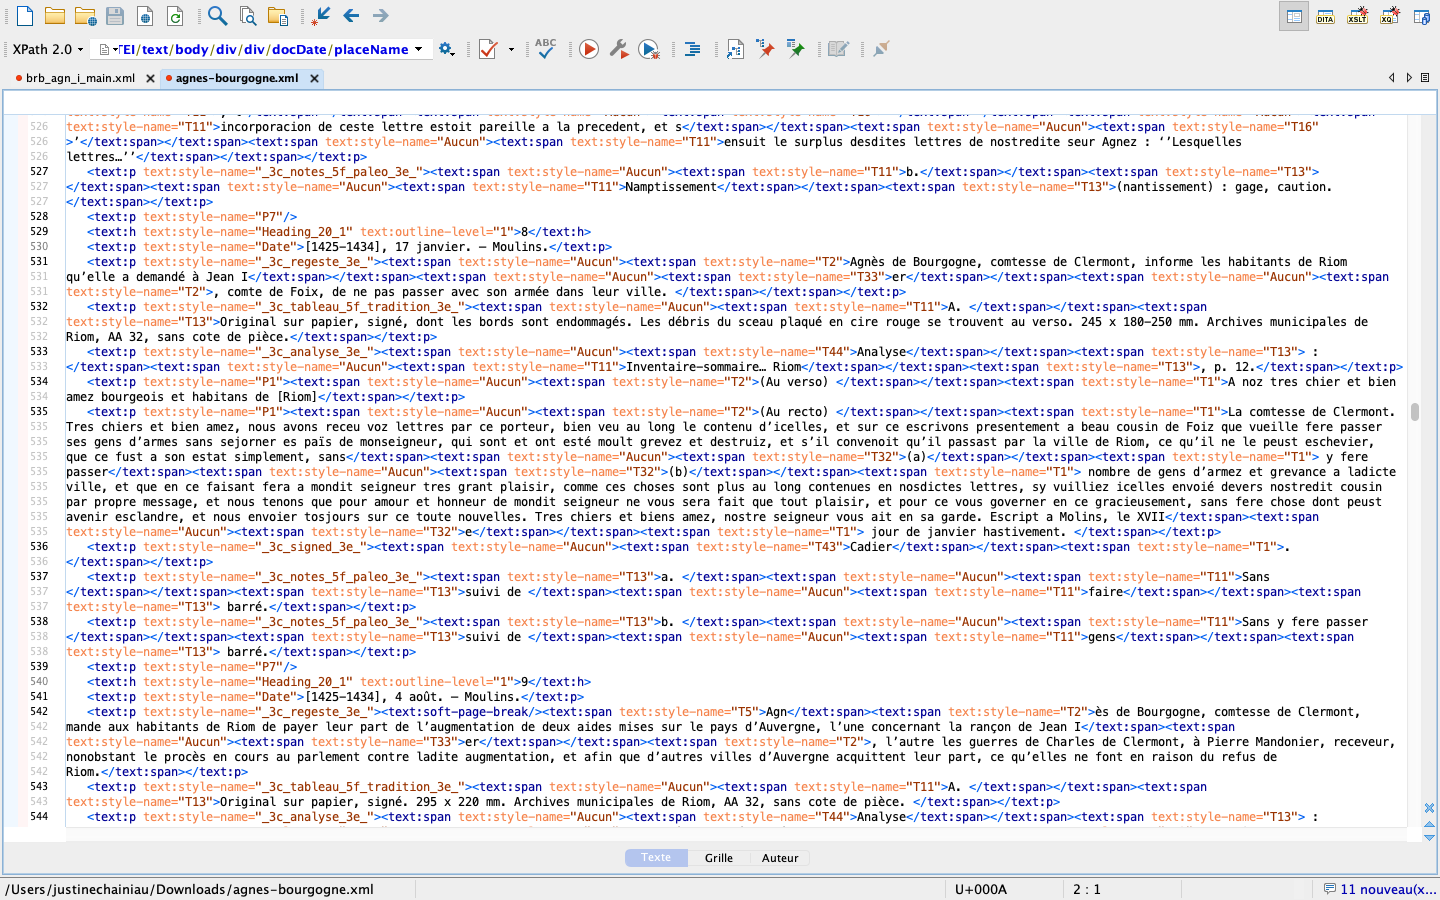
\includegraphics[scale=0.31]{front/images/onlineconvertfree.png}
    \caption{Document XML converti avec \textit{Online ODT converter}.}
    \label{fig:online_odt_converter}
\end{figure}

\par De plus, l’utilisation de ces convertisseurs pose un problème déontologique avec des développeurs non identifiés et des éditeurs peu fiables. Dans le cadre d’un travail scientifique, il est plus pertinent de favoriser les logiciels développés par la communauté scientifique, généralement plus adaptés aux besoins de cette dernière. D'autre part, ces deux premiers logiciels renvoient des fichiers XML, mais pas au standard TEI.

\newpage 

\section{Essais de conversion avec Pandoc}
\label{II.4.2}

\par Ensuite, nous avons testé une conversion avec \textit{Pandoc} : une bibliothèque Haskell permettant de convertir un format de balisage en un autre, et un outil en ligne de commande qui utilise cette bibliothèque\footnote{Pandoc : a universal document converter, en ligne : \url{https://pandoc.org/}.}. Ce convertisseur a été développé par John MacFarlane, un professeur de philosophie, pour la recherche en Sciences humaines et sociales. Il propose de très nombreuses options de conversion entre différents formats de balisage et de traitement de texte, centrées sur la préservation des éléments structurels d’un document. Nous avons pu tester une conversion de ODT vers XML/TEI, qui s’est montrée plus aboutie. 

\begin{figure}[H]
    \centering
    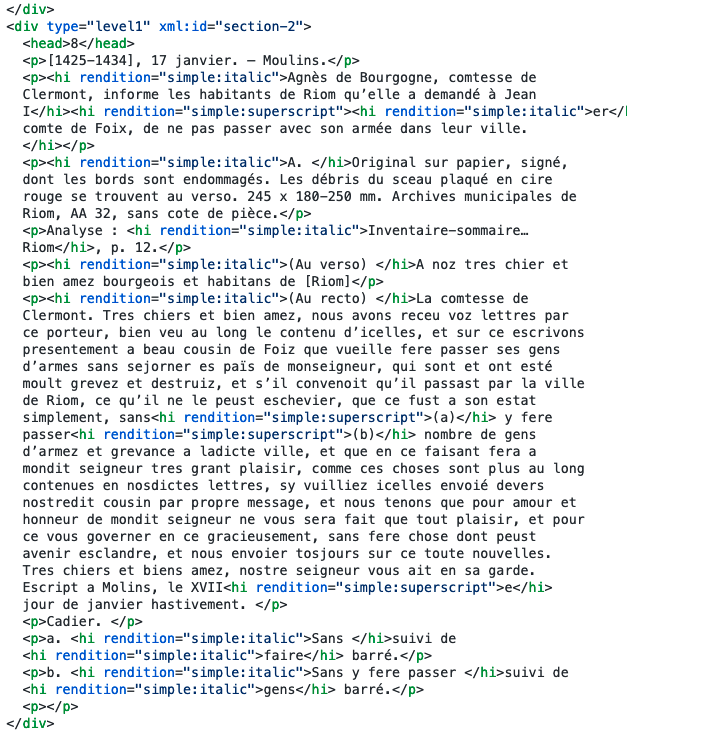
\includegraphics[scale=0.6]{front/images/pandoc_tei.png}
    \caption{Document XML/TEI converti avec \textit{Pandoc}.}
    \label{fig:pandoc_tei}
\end{figure}

\newpage 

\par En effet, cela a permis la génération d’un TEI Header, à compléter. Le niveau de structuration s’est révélé plus lisible, avec l’inscription de chaque acte dans une balise <div>, avec un niveau de titre pour son numéro (<head>). Tous les éléments sont cette fois-ci encodés dans des balises <p>. Cette conversion a fait ressortir l’organisation du document en différenciant les niveaux de titre (numéro, datation) du corps du texte et les notes de bas de page des notes paléographiques. Toutefois, cette reconnaissance manque de précision dans la mesure où elle ne distingue pas les différentes rubriques de l'édition diplomatique qui ont été stylées avec ODT, que sont l’analyse, le tableau de la tradition et le contenu de l’acte, malgré les différents styles qui leur avaient été appliqués. La différenciation des paragraphes ne se fait qu’à partir des graisses (gras, italique) et non des styles ODT appliqués aux différents éléments. Enfin, une conversion d’un docx vers XML/TEI nous a renvoyé une structuration similaire, mais avec un niveau de précision plus fin et une meilleure reconnaissance de la typographie appliquée aux différents éléments du document. Mais cette conversion n’a pas encore permis l’affichage des différents styles comme attributs. 
\newline 

\par Malgré le niveau de description convenable apporté par \textit{Pandoc} dans le cadre d’une conversion de docx vers XML/TEI, nous avons poursuivi nos tests, afin de voir si la hiérarchisation des éléments et la lisibilité pouvaient être améliorées. 

\newpage 

\section{Choix du convertisseur Teinte}
\label{II.4.3}

\par Enfin, nous avons testé le convertisseur \textit{Odette}, pour textes bureautiques (ODT) en TEI\footnote{Frédéric Glorieux, Odette, convertissez vos textes bureautiques (ODT) en TEI, en ligne : \url{http://obvil.lip6.fr/Odette/}.}. \textit{Odette} a été développée par Frédéric Glorieux, ingénieur de recherche en informatique linguistique et documentaire au Labex OBVIL (Observatoire de la vie littéraire) rattaché à la Sorbonne. Le convertisseur produit des documents structurés en XML/TEI via XSLT, de la qualité la plus élevée possible, à partir d’un traitement de texte\footnote{\cite{glorieuxTraitementTextesOdt2015}.}. La conversion permet par exemple d’éditer des pièces de théâtre classique, avec numérotation des vers, paratexte, index ou glossaire, sans perte d’information. La conversion a permis la génération d’un TEI Header à remplir plus développé. La structuration du document est également mieux respectée : chaque acte est encodé dans une <div>. Le numéro d’acte est encodé dans une balise <head>, les différents éléments sont encodés dans des balises <p> avec comme attributs les différents styles appliqués en amont dans le document ODT, permettant ainsi de refléter une hiérarchie et une structure plus précises. De plus, la date de l’acte est encodée dans une balise <dateline>, ce qui montre que le convertisseur a relevé et reconnu cet élément de datation.
\newline 

\begin{figure}[ht!]
    \centering
    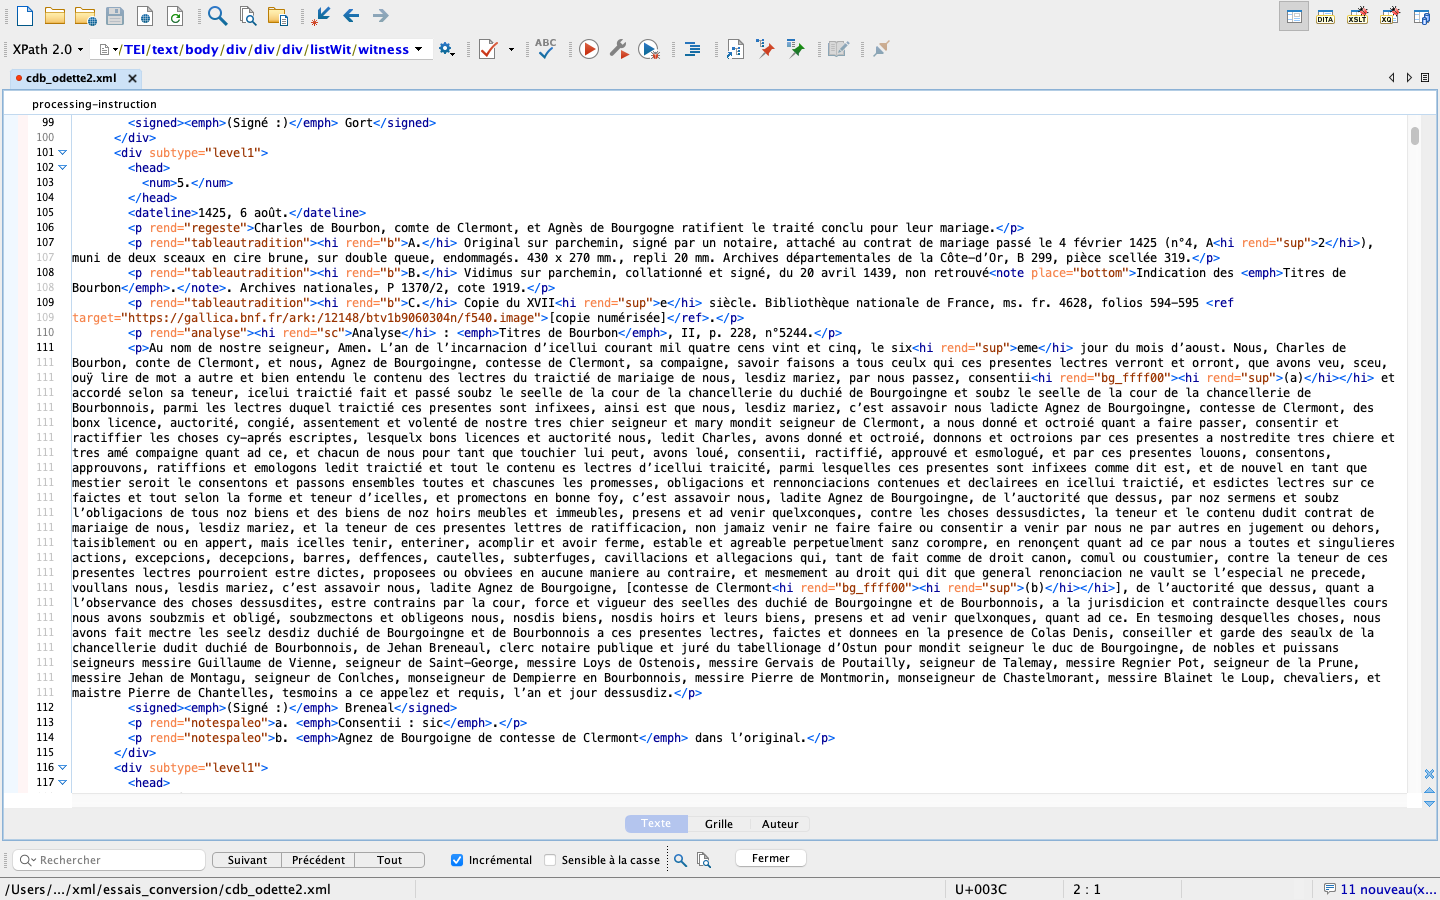
\includegraphics[scale=0.31]{front/images/odette.png}
    \caption{Document XML converti avec \textit{Odette}.}
    \label{fig:odette}
\end{figure}

\newpage 

\par Néanmoins, avant de trancher sur ce convertisseur, il s’agit d’être certain de sa pérennité et de sa stabilité pour une utilisation ultérieure à d’autres corpus dans le cadre du projet Actes Princiers. Afin de s’en assurer, nous avons contacté le développeur d'\textit{Odette}, F. Glorieux. Il nous a parlé de la refonte d'\textit{Odette} dans \textit{Teinte}, une application en développement continu qui permet la conversion de fichiers TEI, Docx, ePub et txt en TEI, Docx, HTML et txt\footnote{Obtic, Teinte, en ligne : \url{https://obtic.huma-num.fr/teinte/}.}. Il s’agit d’un logiciel libre voué à la pérennité dont l'interface a été financée par le Labex ObTIC (Observatoire des textes, des idées et des corpus) rattaché à la Sorbonne. Nous avons tenté une conversion avec \textit{Teinte}, d’un docx vers XML/TEI. Cette dernière s’est révélée très pertinente. Le document XML/TEI retourné est pourvu d’un TEI Header à remplir. Toutefois, ce dernier reste succinct et sera à repenser dans le cadre d’une édition globale des actes princiers. 

\begin{figure}[ht!]
    \centering
    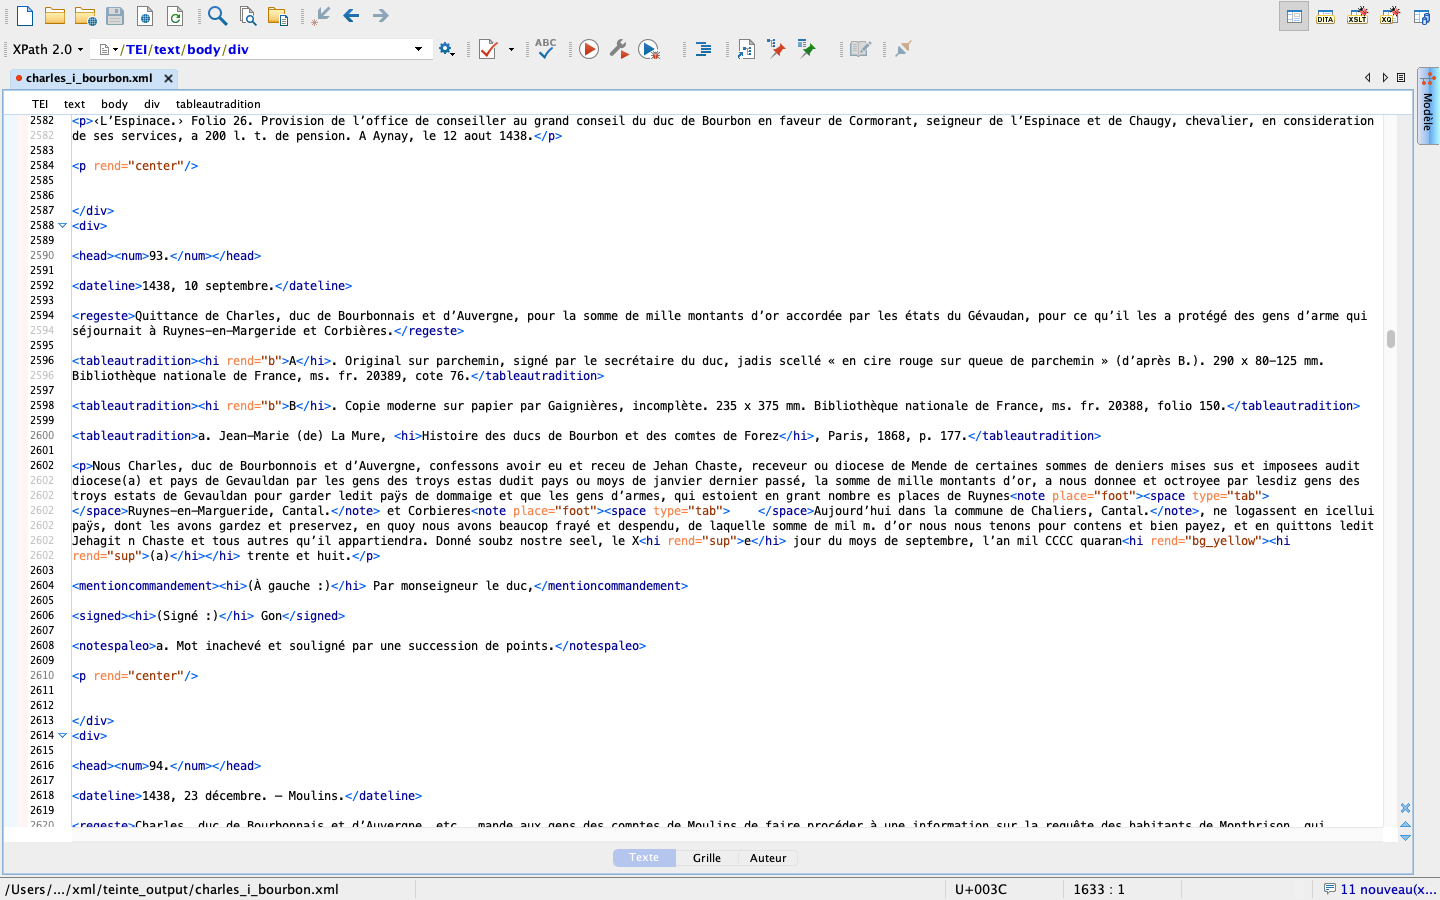
\includegraphics[scale=0.31]{front/images/teinte.png}
    \caption{Document XML/TEI converti avec \textit{Teinte}.}
    \label{fig:teinte}
\end{figure}

\par Comme nous pouvons le voir ci-dessus, le recours à des styles personnalisés et normalisés par un utilisateur sur ODT permet la transformation de ces derniers en éléments (balise avec son contenu textuel). Cela implique une meilleure hiérarchisation des différents éléments diplomatiques. La compréhension est améliorée via la structuration du document et des différentes parties de l'édition dans des balises appropriées. De plus, \textit{Teinte} est un projet développé pour la recherche en sciences humaines et sociales, voué à se pérenniser. Même si le résultat de la transformation ne renvoie pas des balises XML, ces dernières, ainsi que l'organisation du document pourront être repensés et retravaillés. 

\newpage
\thispagestyle{empty}
\mbox{}
\newpage